\chapter{Ancillary Services: Getting Paid to Stand By}
\chaptermark{Ancillary Services}
\label{ch:ancillary}

Everything the book has priced so far is a reaction: the machine watches the price and steps aside when electricity costs more than it earns. Chapter~3 gave a first look at a second set of markets where the product is not energy but readiness. In the ancillary service markets, ERCOT pays resources by the hour simply to stand ready to act, whether or not the call ever comes, and a machine whose whole talent is stepping aside in seconds would seem to be the perfect seller. For one week in 2021, ancillary services were the most lucrative market a megawatt could enter. What happened since is a lesson in how fast open markets eat a good trade, and why the off switch's second income stream is now a complement to the strike price of Chapter~6 rather than a substitute for it.

One unit warning before the tour. Ancillary prices are \glossaryterm{capacity-price}{capacity prices}: dollars per megawatt for each hour of standby, written \$/MW per hour, not dollars per megawatt-hour of energy. A resource earns the clearing price on its committed megawatts every hour it holds the award, on top of whatever it does or does not earn selling or consuming energy. Keep the capacity-price unit separate from the energy-price unit. % src: MCPC definition; the internal AS workbook's own $/MWh axis mislabel is the cautionary case (not cited)

\section{What ERCOT Buys}

ERCOT procures five ancillary services, each a different flavor of readiness, distinguished by how fast it must act and how long it must last \autocite{ercot2026protocols}. % src: ercot2026protocols sec. 2 definitions; tab:as-products
Table~\ref{tab:as-products} lists them with the response clock that defines each one.

\begin{table}[htbp]
  \centering
  \footnotesize
  \setlength{\tabcolsep}{4pt}
  \begin{tabular}{lllr}
    \hline
    \textbf{Service} & \textbf{Acts within} & \textbf{Sustains} & \textbf{2025 avg MW} \\
    \hline
    Reg-Up & 5 s & 30 min & 436 \\
    Reg-Down & 5 s & 30 min & 402 \\
    RRS & 0.25--0.5 s & 15 min to 1 h & 2,739 \\
    ECRS & 10 min & 1 h & 1,416 \\
    Non-Spin & 30 min & 4 h & 2,885 \\
    \hline
  \end{tabular}
  \caption{ERCOT's five ancillary services. Response and sustain requirements from the Nodal Protocols, with the sustain times in force since RTC+B; average procured quantities are day-weighted means computed from ERCOT's published 2025 AS quantities workbook. RRS is provided in three sub-forms with different clocks (see text) \autocite{ercot2026protocols,ercot2025nprr1282,potomac2026somercot,ercotasmeth2025}.} % src: ercot2026protocols sec. 2 (Reg 5 s; FFR 15 cycles; Non-Spin 30 min; ECRS 10 min); secs. 8.1.1.3.1(2), 8.1.1.3.2(4), 8.1.1.3.3(2), 8.1.1.3.4(2) (sustain: Reg 30 min; RRS 30 min if SCED-dispatchable, one hour otherwise, 15 min for FFR from a load; Non-Spin four consecutive hours; ECRS one hour); ercot2025nprr1282 (effective 2025-12-05: Reg and SCED-dispatchable RRS 15 to 30 min, ECRS two consecutive hours to one; sec. 2 and sec. 3.17.4(1) still print ECRS as two consecutive hours); RRS 0.5 s is the load relay's clock (ercotnog2026 sec. 2.3.1.2, as the text below prints it) and governors begin in about 3.5 s (FERCNERCFeb2021 appendix p. 19, chapter 2 sec:inertia); potomac2026somercot p. 38 (LFC signals every 4 s); ercotasmeth2025 workbook (436/402/2,739/1,416/2,885 MW day-weighted means)
  \label{tab:as-products}
\end{table}

Regulation is the fine motor control. ERCOT's Load Frequency Control sends a correction signal every four seconds, and regulation resources must follow it within five, nudging output or consumption up (Reg-Up) or down (Reg-Down) to hold the grid at 60~Hz between economic dispatch runs \autocite{potomac2026somercot,ercot2026protocols}. % src: potomac2026somercot p. 38 (LFC every 4 s); ercot2026protocols sec. 2 (respond within five seconds)

Responsive Reserve is the crash barrier: capacity that arrests a falling frequency in the first seconds after a big generator trips \autocite{ercot2026protocols}. % src: ercot2026protocols sec. 2 RRS definition ("arrest frequency decay within the first few seconds")
It comes in three sub-forms. The first is the primary frequency response of Section~\ref{sec:inertia}, which every generator must be able to provide: its turbine governors begin about three and a half seconds after a trip and feed in more steam or gas as frequency falls, without waiting for any instruction. Storage and controllable load resources provide it too \autocite{FERCNERCFeb2021,potomac2026somercot}. Batteries provide nearly all of the \glossaryterm{fast-frequency-response}{fast frequency response} (FFR), full output within a quarter second of a frequency trigger, sustained at least fifteen minutes, but any load fast enough may qualify for it too \autocite{ercot2026protocols,potomac2026somercot}. % src: FERCNERCFeb2021 appendix E, appendix p. 19 ("conventional generators typically begin their governor response in about 3.5 seconds"), as chapter 2 sec:inertia prints it; ercot2026protocols sec. 2 FFR definition ("provision by a Resource"; 15 cycles = 0.25 s; sustain 15 min), sec. 3.17.2(3)(b) (RRS from Resources capable of FFR), sec. 8.1.1.3.2(4) ("non-Controllable Load Resources qualified to provide FFR", 15 min); potomac2026somercot p. 132 (FFR "provided almost exclusively by batteries"; PFR "provided by generators, storage resources, and controllable load resources") and p. 38 (PFR, "which all generators must be able to provide")
And loads provide the bluntest form of all: an \glossaryterm{under-frequency-relay}{under-frequency relay} (UFR), a hardware tripwire that disconnects the whole site within half a second when frequency falls to its setting, with nothing in software between the frequency and the breaker \autocite{ercotnog2026}. % src: ercotnog2026 sec. 2.3.1.2 (total interruption within 30 cycles = 0.5 s incl. relay and breaker); trip setting no lower than 59.70 Hz

ECRS, launched June 10, 2023 as the first new daily procured service in more than twenty years, is the ten-minute reserve: capacity ERCOT can call to restore the crash barrier after it has been used, sustained for at least an hour (two hours until RTC+B cut it in December 2025) \autocite{ercotecrs2023launch,potomac2023som,ercot2025nprr1282}. % src: ercotecrs2023launch ("first daily procured Ancillary Service introduced to the ERCOT market in more than 20 years"); potomac2023som p. 96 (go-live June 10, 2023); ercot2026protocols sec. 2 (10 min), secs. 8.1.1.2.1.7(3), 8.1.1.3.4(2) (maintain the award at least one hour; sec. 2 and sec. 3.17.4(1) still print two consecutive hours); ercot2025nprr1282 (two consecutive hours to one hour, eff. Dec 5, 2025)
Non-Spin is the slow reserve: thirty minutes to arrive, four hours of endurance, the service that covers a forecast bust rather than an instant failure \autocite{ercot2026protocols}. % src: ercot2026protocols sec. 2 Non-Spin definition (30 min, four consecutive hours)

Two facts about this shopping list matter for everything that follows. First, it is large: about 7,900~MW of standby held every average hour of 2025, and the market monitor complains, year after year, that ERCOT buys roughly twice the reserves a reasonable reliability standard would require \autocite{ercotasmeth2025,potomac2026somercot}. % src: ercotasmeth2025 workbook (sum of the five day-weighted means = 7,878 MW); potomac2026somercot pp. 3, 39 ("more than double")
Second, loads are welcome nearly everywhere in it. Every service except Regulation can be provided by a load with nothing more sophisticated than an on-off switch, and every service on the list, Regulation included, can be provided by a load that qualifies as controllable \autocite{ercot2026protocols}. % src: ercot2026protocols sec. 3.6.1 (Load Resource participation by service); sec. 3.16 caps
ERCOT pays the same clearing price whether readiness comes from a turbine that can spin up or a mining hall that can go quiet.

A sixth service is on its way. The Dispatchable Reliability Reserve Service, a slower reserve that must reach its level within two hours and hold it for four, was approved in July 2026 but waits on system changes that ERCOT's project list targets for late 2028; only generators may sell it, and its arrival cuts Non-Spin's endurance to two hours \autocite{ercot2026nprr1309,ercot2026rrprojects}. % src: ercot2026nprr1309 (PUCT approved July 9, 2026, effective upon system implementation; its gray boxes in ercot2026protocols Aug 1, 2026: sec. 2 DRRS definition; new sec. 3.17.5, capacity from Off-Line or On-Line Generation Resources that ramp within two hours and run at least four consecutive hours; sec. 2 Non-Spin definition, sec. 3.17.3(1)(a)(ii),(b)(ii) and sec. 8.1.1.3.3(2), four consecutive hours to two; PUCT Report 1309NPRR-35, whose justification says the NPRR was developed pursuant to PURA 39.159(d), statute not read); ercot2026rrprojects (project 575-01 NPRR1309, status Initiation, target end November 30, 2028)

\section{What Standing By Paid, 2021 to 2026}

Figure~\ref{fig:as-history} shows the five clearing-price histories on one log scale, and Figure~\ref{fig:as-standing-revenue} compresses each year into a single number: the \glossaryterm{standing-revenue}{standing revenue}, what one megawatt earned by holding the award through every hour of the year, before any energy consequences. It is a ceiling, not a forecast: it assumes an award in every hour at the day-ahead clearing price, with no QSE fee, no deployment cost and no failed-performance event.

\begin{figure}[htbp]
  \centering
  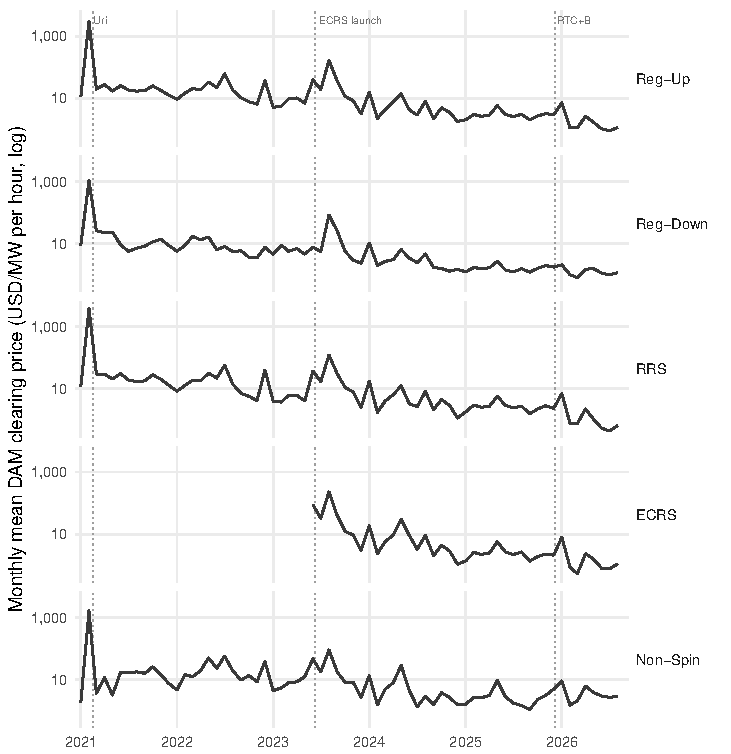
\includegraphics[width=\textwidth]{images/as_price_history}
  \caption{
    Monthly mean day-ahead clearing prices for the five ancillary services, 2021 to mid-2026, log scale. The February 2021 spike is Winter Storm Uri; ECRS appears at its June 2023 launch and spends its first year as the most expensive product on the board; everything decays toward single digits as batteries flood in; RTC+B changes the market's plumbing in December 2025. Prices below \$0.10 are drawn at \$0.10. % fig-src: analysis/figures/fig_ch7_as_history.R on analysis/data/ercot_dam_as_mcpc.csv.gz
  }
  \label{fig:as-history}
\end{figure}

Act one is Uri. During the February 2021 emergency, day-ahead ancillary prices cleared above \$25,000 per megawatt for single hours, nearly three times the era's \$9,000 system-wide offer cap, because the clearing algorithm priced the opportunity cost of scarce capacity without any cap of its own \autocite{potomac2021som}. % src: potomac2021som p. vi ("MCPCs ... in excess of $25,000 per MW"; DAM algorithm opportunity-cost design)
The market monitor called the outcome a roughly \$2~billion overvaluation of ancillary services, and the rules were changed within months: ancillary prices are now capped at the system-wide offer cap, and the cap itself was cut to \$5,000 the following January \autocite{potomac2021som}. % src: potomac2021som p. vi ($2B overvaluation; NPRR1080 June 2021; HCAP to $5,000 effective Jan 1, 2022)
For sellers, that one storm made the year. A megawatt that held RRS through all of 2021 collected about \$2.7~million, and 91~percent of it accrued in Uri week alone. % src: fig_ch7_as_history.R console (RRS 2021 total $2,735,205; Uri week Feb 14-20 $2,485,794 = 91%)

Act two is the ECRS misadventure. The new ten-minute product launched in June 2023 into a hot summer, and ERCOT held it back so firmly during tight hours that the market behaved as if the system were short when it was not. The market monitor concluded that the way ECRS was procured and withheld created artificial shortage pricing that roughly doubled real-time energy prices from June through December and added more than \$12~billion of real-time market costs \autocite{potomac2023som}. The service itself cost more than \$600~million to procure and bought a computed reliability benefit of about \$12~million, a fifty-to-one ratio of cost to value. % src: potomac2023som pp. ii, ix, 11 (doubled RT prices Jun-Dec; >$12B excess; $600M procurement vs $12M value = 50x)
The market monitor put ECRS's 2023 average near \$77 per megawatt per hour of standby, over triple the RRS average, and a megawatt standing in the product from launch day collected \$286,000 in seven months \autocite{potomac2023som}. % src: potomac2023som p. ii ($76.77, over triple RRS; the IMM average is not the simple hourly mean, which is $58.15 per fig_ch7_as_history.R console); fig_ch7_standing_revenue.R console (ECRS 2023 partial-year $286,136)


Act three is the flood, and Chapter~6 already introduced its protagonist. Batteries are nearly ideal ancillary machines, and as their fleet quadrupled they moved into these markets first: the monitor's phrasing is simply that storage \emph{flooded} the ancillary markets and prices fell \autocite{potomac2026somercot}. % src: potomac2026somercot p. 22 ("As ESRs have flooded the AS markets, AS prices have fallen"); quadrupled = 4.4 -> 18.1 GW per ch6 fig_ch6_batteries.R (EIA-860M July 2026)
ECRS collapsed from about \$77 to under \$10 per megawatt per hour in a single year, a drop the market monitor puts down to new supply, batteries above all \autocite{potomac2024som}. % src: potomac2024som pp. ii, vi ($76.77 -> $9.62; "This drop was caused by an increase in supply, particularly from energy storage resources (ESRs)")
ERCOT's own attempt at a repair, formal triggers for releasing the reserve to the market, was rejected by the commission in July 2024; ERCOT applied the triggers anyway, without the rule's \$750/MWh floor on the reserve's energy offers, and the monitor judged the method flawed, since it let artificial shortages set in before the reserve was released \autocite{ercotnprr1224,potomac2024som}. % src: ercotnprr1224 (posted March 27, 2024, urgent; manual ECRS release when the power balance violation is at least 40 MW for ten consecutive minutes; ECRS Energy Offer Curves floored at $750/MWh; Board recommended June 18, 2024; PUCT rejected July 25, 2024); potomac2024som pp. xxi, 13 (PUCT rejection July 2024, then "ERCOT still implemented the deployment process proposed by NPRR 1224, but without the $750 per MWh energy offer floor"; "effectively forcing the real-time market into artificial shortage conditions before releasing ECRS"), p. 14 (3 of 24 costly 2024 events had NPRR 1224 deployments)
In 2025 every product fell again, and the total cost of all five services dropped to 39 cents per megawatt-hour of load served, the lowest since 2020, down from \$29.59 in Uri's year \autocite{potomac2026somercot,potomac2021som}. % src: potomac2026somercot p. 3 ($0.39/MWh load, -60%, lowest since 2020); potomac2021som p. 43 ($29.59 in 2021)

\begin{figure}[htbp]
  \centering
  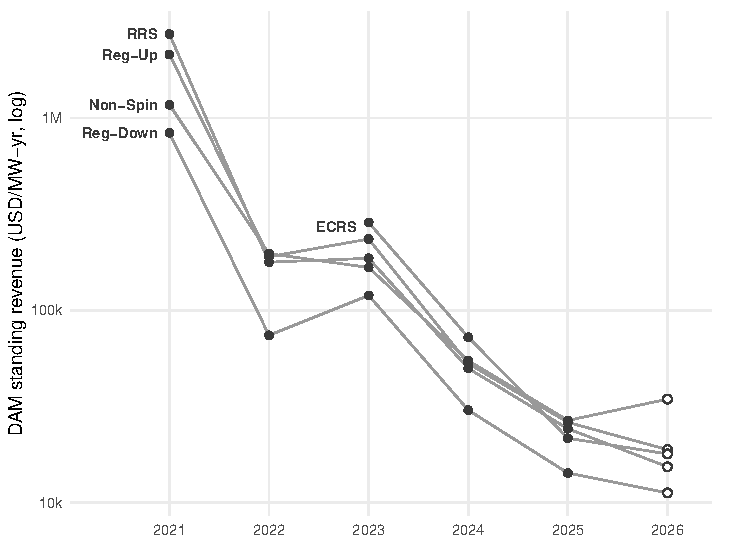
\includegraphics[width=\textwidth]{images/as_standing_revenue}
  \caption{
    Standing revenue by product and year: what one megawatt earned by holding each award through every hour, log scale. RRS fell from \$2.74~million per megawatt-year in 2021 to \$24,000 in 2025, a 113-fold decline; the whole product stack, four products in 2021 and five by 2025, fell 61-fold. The 2026 run rate is lower again for every product except Non-Spin, the only one rising. ECRS's 2023 is a partial year from its June launch; the 2026 open markers are the total to date, annualized. % fig-src: analysis/figures/fig_ch7_standing_revenue.R; console: RRS 2,735,205 -> 24,168; stack 6,886,902 -> 112,749
  }
  \label{fig:as-standing-revenue}
\end{figure}

Add the products together, a sum no single megawatt could collect, and the whole product stack fell from \$6.9~million per megawatt-year at the 2021 extreme to about \$113,000 in 2025, a 61-fold compression. % src: fig_ch7_standing_revenue.R console (stack 2021 $6,886,902; 2025 $112,749)
The same force that squeezed the daily price spread in Chapter~6 squeezed the standing revenue here, and harder, because ancillary markets are small: a few thousand megawatts of demand against eighteen gigawatts of batteries hunting for work. Batteries' own ancillary revenue fell by more than a third in 2025 even as their fleet grew by 80~percent; they saturated their first market and moved on to arbitrage \autocite{potomac2026somercot}. % src: potomac2026somercot pp. 22-23 (AS revenue fell >37%; ESR fleet +80%); 18 GW = 18.1 GW nameplate mid-2026 per ch6 fig_ch6_batteries.R (EIA-860M July 2026)

\section{Why a Flexible Load Should Still Care}
\label{sec:as-why-care}

At 2025 prices, is any of this worth a miner's attention? Run the arithmetic from the miner's chair. A single megawatt standing in ECRS through 2025 earned about \$22,000; in Non-Spin, about \$27,000. % src: fig_ch7_standing_revenue.R console (ECRS 2025 $21,579; Non-Spin $26,699)
Against the \$370,000 that megawatt spends on index power in a year, that is a six or seven percent rebate on the power bill, roughly half of what the Chapter~6 strike earned the older fleet, for a capability the machines already possess. % src: ch6 analysis/checks/ch6_contract_pnl.R (RT index $369,454/MW-yr); fig_ch6_strike.R ($49,116 S19j Pro strike value)
Because that is the point worth stressing: \emph{the machines need nothing new to sell readiness}. The reflex of Chapter~5 already watches prices in real time and already pauses the site in seconds; ancillary participation rents that existing reflex to the grid operator for hours when it would otherwise sit unused. Deployments are rare, and between them the machines simply mine. The standing revenue stacks on top of mining margin.
The market interface is another matter, and a project in its own right: a Qualified Scheduling Entity to represent the site, a telemetry link, a qualification test and, for the simplest form of Responsive Reserve, a relay \autocite{ercot2026protocols}. % src: ercot2026protocols sec. 16.5.1.1 (QSE designation), sec. 8.1.1.1(1),(4) (qualification criteria; a Load Resource providing AS in Real-Time needs ESI ID registration by its QSE and telemetry installed and tested between QSE and ERCOT), sec. 3.17.2(3)(c) (RRS from Load Resources controlled by high-set under-frequency relays); ercotnclrtest2026, ercotclrtest2024 (qualification tests)

Miners noticed this long before the batteries arrived. In June 2020 Lancium and MP2 Energy announced what they called ERCOT's first controllable resource made of load alone, with no generation behind it, at a Big Spring, Texas, data center run by Compute North, a provider of data infrastructure for cryptocurrency mining \autocite{lancium2020clr}. % src: lancium2020clr (PR Newswire, June 19, 2020: "the first successful load-only Controllable Load Resource (CLR) designation by the Electric Reliability Council of Texas", "a first in ERCOT for a load only and without generation", "achieved at the Compute North Data Center in Big Spring, TX"; Compute North is an industry leader in data infrastructure "for blockchain, cryptocurrency mining and the broader high-performance computing space"); the vendors' claim, no ERCOT record of the first CLR found (ercotlaar, potomac2026somercot searched)
By 2025 the market monitor reported that all twelve resources registered in ERCOT's most demanding load category are cryptocurrency mines, and mining demand on the system peaked at roughly 4,600~MW that year \autocite{potomac2026somercot}. % src: potomac2026somercot p. 28 ("In 2025, all 12 registered CLRs are cryptocurrency mines"), p. i ("Aggregate demand for crypto-currency mining was approximately 4,600 MW in 2025"), p. 31 ("peak demand reaching 4,600 MW in 2025")
That is mining alone, at its 2025 peak, and a different count from Chapter~3's 5,800~MW, which adds up the large loads of every industry energized through ERCOT's large-load program, each at its own highest draw. % src: chapter 3 sec:miners-ercot (ercot2026llistatus slide 3: Observed Energized, all project types, "all time non-simultaneous peak load consumption"); potomac2026somercot p. 31 (2025 peak of mining demand)
ERCOT's own qualification paperwork now lists ``crypto mining'' and ``AI data center'' as example load types on the application form, and ERCOT went as far as licensing one mining company's patents, at no cost, so that every registered controllable load could participate without infringement risk \autocite{ercotclrtest2024,ercotlaar}. % src: ercotclrtest2024 sec. 2.2 (one-line diagram form); ercotlaar (ERCOT-Lancium patent license, all registered CLRs deemed sublicensees)
The rest of this chapter explains what that demanding category is, what joining it takes, and why, in 2025, many miners quietly stepped back out of it.

\section{The Controllable Load Resource}
\label{sec:clr}

ERCOT's rulebook recognizes two ways for a load to sell readiness, and the difference is a hierarchy of trust \autocite{ercot2026protocols,potomac2024som}. % src: ercot2026protocols sec. 2 definitions; potomac2024som (two types of load resources)

A load resource is any load registered to provide ancillary services. In its basic, non-controllable form (ERCOT's test procedures call it an NCLR), its instrument is the under-frequency relay: a hardware setting, armed when the site holds an RRS award, that trips the breaker within half a second when frequency falls to its setting, which may be set no lower than 59.70~Hz \autocite{ercotnclrtest2026,ercotnog2026}. % src: ercot2026protocols sec. 2 (Load Resource definition); sec. 3.6.1(1)(a)(v)-(vi) (the Protocols write "Load Resource that is not a CLR"; NCLR occurs in none of secs. 2, 3, 6, 8 or 16); ercotnclrtest2026 ("Non-Controllable Load Resources (NCLRs)"; UFR no lower than 59.70 Hz, relay delay max 20 cycles); ercotnog2026 sec. 2.3.1.2 (30 cycles total)
It can also take a ten-minute phone-call-style dispatch for ECRS, relay armed or not, or a thirty-minute one for Non-Spin, but only with the relay disarmed, so never in the same interval as RRS \autocite{ercot2026protocols,ercotnclrtest2026}. % src: ercot2026protocols secs. 3.17.3(1)(c), 3.17.4 (non-CLR Load Resources: ECRS on ten minutes' notice, Non-Spin within 30 minutes); sec. 3.6.1(1)(a)(iv)-(vi) (ECRS from a Load Resource that "may or may not be controlled by high-set under-frequency relay"; Non-Spin only from a Load Resource "that is not controlled by under-frequency relay"; "cannot simultaneously provide Non-Spin and RRS in Real-Time"); ercotnclrtest2026 sec. 2.3 (UFR "Armed" to carry RRS, "Unarmed" to carry Non-Spin, either for ECRS alone); test pass criteria
What it cannot do is modulate: it is a binary device from the grid's point of view, on or tripped.
Its standard is as plain as its relay: such a load fails if it delivers less than 95~percent of what ERCOT calls for within ten minutes (thirty for Non-Spin), whether the call is real or, for RRS and ECRS, one of ERCOT's unannounced interruption tests. Two failures in any rolling year cost it its qualification, with a six-month wait before it may reapply \autocite{ercot2026protocols}. % src: ercot2026protocols sec. 8.1.1.1(8)-(9) (Load Resources excluding CLRs providing RRS or ECRS: under 95% of the award within ten minutes of an ERCOT Dispatch Instruction is a failure; two failures, in a deployment event or in a Load interruption test at a time known only to ERCOT and the TSP, within any rolling 365-day period disqualify; reapply after six months with a corrective action plan and a new test); sec. 8.1.1.4.3(5) (Non-Spin from a Load Resource that is not a CLR: under 95% of the instruction within 30 minutes is a failure; two failures in any rolling 365 days disqualify; reapply after six months); ercotrtcbloadres2025 slide 13 (unchanged by RTC)

A Controllable Load Resource (CLR) is, in the rulebook's own words, ``a Load Resource capable of controllably reducing or increasing consumption under Dispatch control by ERCOT'' \autocite{ercot2026protocols}. % src: ercot2026protocols sec. 2 (CLR definition, verbatim)
A CLR receives a \glossaryterm{base-point}{base point}, a target consumption level, from the same five-minute economic dispatch that steers every power plant in Texas, and ERCOT scores its compliance against that target every interval \autocite{ercot2026protocols}. % src: ercot2026protocols sec. 6.5.7.4 (Base Points to CLRs each SCED run); sec. 8.1.1.4.1 (CLREDP metric per 5-min interval)
In exchange, the full product shelf opens: a CLR can sell Regulation, RRS, ECRS, and Non-Spin, while the relay-only load is shut out of Regulation entirely and capped as a class, at 60~percent of the RRS requirement together with the batteries' FFR, and at half of the ECRS requirement \autocite{ercot2026protocols}. % src: ercot2026protocols sec. 3.6.1 (services by type); sec. 3.16(4) (60% RRS cap on UFR+FFR); sec. 3.16(7) (50% ECRS cap on non-CLR loads)

The requirements climb with the privileges. A CLR must respond to frequency like a power plant's governor: a \glossaryterm{frequency-deadband}{frequency deadband} no wider than plus or minus 0.036~Hz, five percent droop (the standard slope that ties the size of the response to the size of the frequency error), response demanded automatically whenever frequency wanders outside the band \autocite{ercotnog2026}. % src: ercotnog2026 secs. 2.2.7-2.2.8 (CLR deadband 0.036 Hz, droop 5%)
For a mining site this means the control system does not merely pause machines on command; it continuously trims kilowatts against a 60.000-hertz target the way a turbine trims steam. Qualification is a proving ground with several stations: a dispatch-following test in which ERCOT drives the site between its maximum and minimum consumption inside single five-minute intervals, a frequency-response self-test, and a separate test for each service the site wants to sell, all using real demand response rather than paperwork \autocite{ercotclrtest2024}. % src: ercotclrtest2024 secs. 2.3-2.5 (SCED test: to MPC, hold 4 min, ramp to LPC within one SCED interval; PFR self-test); ercot2026protocols sec. 8.1.1.2(13) (tested using actual demand response)
The frequency duty is set to narrow. A rule change the commission approved in November 2024, which ERCOT schedules for early 2027, keeps governor-style response only for the CLRs qualified to sell Regulation or Responsive Reserve; a CLR without it may still follow base points and sell ECRS and Non-Spin \autocite{ercot2024nprr1244,ercotrtcbloadres2025,potomac2026somercot,ercot2026rrprojects}. % src: ercot2024nprr1244 (PUCT approved Nov 21, 2024, effective upon system implementation; PUCT Report 1244NPRR-11: "maintains existing provisions that require a Controllable Load Resource to be capable of providing PFR in order to be eligible to provide Regulation Service and/or RRS but eliminates this requirement as to a Controllable Load Resource that provides ECRS"); its gray boxes in ercot2026protocols sec. 3.6.1(1)(a)(iv) and sec. 8.5.2.1(1) (Aug 1, 2026; the 8.5.2.1(1) box is shared by NPRR995 and NPRR1244; today 8.5.2.1(1) requires PFR of all CLRs, and 3.6.1(1)(a)(v) never tied Non-Spin to it); ercotnog2026 sec. 2.2.8(1), gray box of NOGRR263 (droop for "CLRs that are capable of providing Primary Frequency Response"; performance for a "CLR qualified for Regulation Service and/or RRS"); ercotrtcbloadres2025 slides 9, 12 ("the CLRs that are qualified for Regulation and/or RRS"); potomac2026somercot p. 30 n. 15 (NPRR1244 with NPRR1188 in January 2027); ercot2026rrprojects (project 539-01 NPRR1188 NPRR1244, status Execution, target end March 1, 2027; the April 14, 2026 edition of the workbook had January 1, 2027)
A freshly qualified CLR is trusted with Responsive Reserve equal to only 20~percent of its maximum consumption until it demonstrates a steeper response \autocite{ercotclrtest2024}. % src: ercotclrtest2024 sec. 2.8 (default RRS qualification 20% of MPC)
And the standard, once earned, must be kept, though by a different yardstick from the relay-only load's: in at least 85~percent of the month's five-minute intervals, the site's consumption must land within ERCOT's posted tolerance of its base point, and during any declared energy emergency it may miss that tolerance in no more than three five-minute intervals. ERCOT reports a shortfall to the \glossaryterm{reliability-monitor}{reliability monitor} and may revoke the qualifications of a site that keeps falling short \autocite{ercot2026protocols}. % src: ercot2026protocols sec. 8.1.1.4.1(2),(8)(a) (CLREDP each five-minute interval with status ONL; below the greater of X% or Y MW in 85% of the month's intervals; non-compliance reported to the Reliability Monitor), (8)(b)(i) (in intervals in which ERCOT has declared EEA Level 1 or greater, "A CLR cannot fail this criteria more than three five-minute clock intervals during which EEA was declared", measured separately for each EEA and reported to the Reliability Monitor); sec. 8.1.1.4.1(10) (X and Y posted on the ERCOT website); sec. 8.4(2) (AS qualifications revocable for continued material non-performance); sec. 8.1.1.1(9) (the two-failure rule excludes CLRs); sec. 2 (Reliability Monitor selected by the PUCT)
The reliability monitor checks compliance with grid reliability rules and supports the commission's enforcement work. ERCOT performs that role under the commission's direction; Potomac Economics, the market monitor, examines market conduct and design \autocite{ercot2026reliabilitymonitor,potomac2026somercot}.

The caps and that 20~percent decide what the prices of Section~\ref{sec:as-why-care} leave out: how much a load can sell at all. In 2025, 7,568~MW of relay-only loads qualified for RRS and supplied only 1,480~MW on average: ERCOT keeps at least 1,365~MW of RRS for primary frequency response, relay-only loads and the batteries' FFR may take the rest up to 60~percent of the RRS requirement, and when their limit binds, as it usually does, ERCOT scales their awards down pro rata \autocite{ercot2026protocols,ercotasmeth2025,potomac2026somercot}. % src: ercot2026protocols sec. 3.16(4) (monthly PFR minimum; the rest open to all qualified Resources, UFR Load Resources and FFR limited to 60% of the RRS requirement), (6) (Load Resource RRS limited to the lesser of the 60% limit and the paragraph (4) limit); ercotasmeth2025 methodology (PFR minimum not less than 1,365 MW; DAM limits UFR plus FFR to 60%) and workbook sheet 2025 RRS Table (LRs = total RRS - 1,365 MW PFRS in every month-hour: 935 to 1,780 MW, 40.7 to 56.6% of RRS, day-weighted mean 1,374 MW against a 60% cap of 1,644 MW, so the PFR floor and not the 60% cap set the limit throughout the 2025 plan; recomputed 2026-09-27 from the archive fetched that day); potomac2026somercot p. 37 (NCLRs provided 1,480 MW of RRS on average in 2025), p. 43 (7,568 MW of NCLRs qualified; the 1,365 MW PFR floor is "one reason for this gap"), p. 45 (ERCOT "prorates UFR and FFR awards when the combined limit is binding"), p. 46 (UFR volumes fell from 2024 to 2025, "The main driver was the increase in the minimum PFR volume requirement from 1,185 MW to 1,365 MW"), p. 132 (the UFR and FFR limit "usually binds", leaving "a surplus of offers for both FFR and UFR")
Half of ECRS, about 710~MW, was open to relay-only loads; they supplied 190~MW. CLRs face no class cap, and sold 9~MW of RRS, 11~MW of ECRS and 58~MW of Non-Spin on average \autocite{ercot2026protocols,potomac2026somercot}. % src: ercot2026protocols sec. 3.16(7) (Load Resources excluding CLRs limited to 50% of the ECRS requirement); 0.5 x 1,416 MW (tab:as-products) = 708 MW; potomac2026somercot p. 37 (NCLRs 190 MW of ECRS; CLRs 9 MW RRS, 11 MW ECRS, 58 MW NSRS), p. 44 ("no cap on the share of responsive reserves provided by CLRs")
A 67~MW site like Chapter~9's would be a tenth of the relay-only loads' ECRS allowance, and as a new CLR could sell Responsive Reserve on about 13~MW, a fifth of its connection. % src: chapter 9 sec:stack-site, its first sentence (30.68 + 36.45 = 67.13 MW at stock power, the ledger's whole site, as that line's source note gives it), and its paragraph "The connection binds" (the 67.13 MW connection caps the site's consumption); 67.13 / 708 = 9.5%; 0.2 x 67.13 = 13.4 MW (ercotclrtest2024 sec. 2.8, default RRS 20% of MPC); flat out at 74.10 MW with no connection cap it would be 14.8 MW; the connection is the maximum the site can consume, so 20% of it is the printed base
In my reading, the first question for a QSE is how many megawatts will clear, and only then what each one earns.

None of this is exotic for a mining fleet. Chapter~5's loop already holds a power target, pauses and resumes a machine in about 30 seconds, and moves it in seconds between targets it holds a saved profile for (Chapter~5 gives the profile rule), so a fleet follows any dispatch level by pausing and resuming individual machines. The CLR requirements mostly ask the loop to point that reflex at grid frequency and dispatch instructions instead of only at price. % src: chapter-5.tex secs. 5.1-5.2 (pause and resume ramp in about 30 s each, braiinsacademyramping, read 2026-09-27; was "in seconds", per the author 2026-08-28; a target with a saved tuning profile is applied again without a new run, only that exact target: braiinsacademyautotuning, braiinsacademydps); narrowed from "already actuates in seconds", which did not hold for a target's first tuning run, in the wording the author approved on 2026-09-26 (STATUS open item 5)
The genuinely new work is in the wires between the site and the market.

\section{The Plumbing: Telemetry, QSEs, and What It Costs}

A mining site cannot talk to ERCOT directly. Every resource must be represented by a Qualified Scheduling Entity (QSE), the licensed intermediary that submits offers, receives dispatch, and settles every payment on the resource's behalf; designating one is a registration requirement, not an option \autocite{ercot2026protocols}. % src: ercot2026protocols sec. 2 (QSE definition), sec. 16.5.1.1 (mandatory QSE designation)
The physical chain runs in three links. At the site, a telemetry gateway (in substation language, a remote terminal unit) reads the meters and breaker states. It reports over a secured private line to the QSE's control center, because ERCOT requires that last mile to be a protected network rather than the open internet \autocite{ercotnog2026}. % src: ercotnog2026 sec. 7.1.2 (QSE collects SCADA for Resources; Secure Private Network requirement for the QSE-to-site leg)
The QSE's control system then speaks to ERCOT over the grid world's standard control-room protocol, ICCP, across ERCOT's own private wide-area network, using routers that ERCOT itself supplies and manages at the QSE's premises \autocite{ercotnog2026,ercoticcp2025}. % src: ercotnog2026 secs. 7.1.1, 7.3 (ICCP over the ERCOT WAN; ERCOT-supplied premises equipment); ercoticcp2025 (ICCP = TASE.2 standard)

What flows through that pipe is specific and fast. Upward, every two seconds: the site's consumption, its operating limits, its relay and breaker status, its ramp rates, all to three percent accuracy or better \autocite{ercoticcp2025,ercot2026protocols}. % src: ercoticcp2025 Tables 28/31 (2-second frequency per Load Resource point); ercot2026protocols sec. 6.5.5.2(6),(10) (telemetry list; 3% accuracy)
Downward: a base point from every five-minute dispatch run, regulation signals every four seconds for sites selling that product, and deployment instructions when the grid actually needs the reserve \autocite{ercot2026protocols,potomac2026somercot}. % src: ercot2026protocols sec. 6.5.7.4 (Base Points over ICCP); potomac2026somercot p. 38 (LFC every 4 s)
Once a month, ERCOT reconciles the telemetry against the settlement meter, so the stream that earns the money is audited against the stream that pays the bills \autocite{ercotnog2026}. % src: ercotnog2026 sec. 7.3.3(3) (monthly telemetry-vs-settlement-meter check)

What does the apparatus cost? ERCOT's own price list gives: \$500 to register a load resource, \$500 for a QSE application, a private-network hookup whose ERCOT-side cost is capped at \$7,000 to install and \$450 a month to run, no charge at all for the qualification tests, and a system administration fee of 61 cents per megawatt-hour that is already embedded in every power bill in the state \autocite{ercotfeeschedule2025,ercotsaf2026}. % src: ercotfeeschedule2025 ($500 LR registration; $500 QSE application; WAN <= $7,000 + $450/month); ercotsaf2026 ($0.61/MWh from Jan 1, 2026)
Registration takes a minimum of 45 days, and a new site can operate under a provisional qualification for its first 90 days \autocite{ercotlaar,ercot2026protocols}. % src: ercotlaar (45-day minimum lead time); ercot2026protocols sec. 8.1.1.1(4) (90-day provisional qualification)
The real costs live elsewhere, and they are commercial rather than tariffed. The QSE's fee, the telemetry gateway and its integration have no public price: no QSE publishes a rate card, no miner's securities filings disclose one, and this book will not invent a number where none can be sourced. Get them quoted. % src: verified negative finding (2026-08-30 source sweep): no citable public QSE fee, RTU, or integration cost exists; SEC filings mention QSEs only in passing
Ask the QSE for its retainer, its fee per megawatt and the credit support it will require: ERCOT makes a QSE answer for every settlement charge of its sites, reserves included, and post security, such as a letter of credit, covering its estimated exposure \autocite{ercot2026protocols}. % src: ercot2026protocols sec. 2 (Counter-Party: a single Entity that is a QSE and/or a CRR Account Holder), sec. 16.2.1(1)(k) ("financially responsible for payment of Settlement charges for those Entities it represents"), sec. 16.11.1(1) (Financial Security at all times at or above TPE), sec. 16.11.3(1)(a)-(c) (an unconditional, irrevocable letter of credit, a surety bond or Cash Collateral), sec. 16.11.4.3.2(1)(g)-(k) (the Real-Time Liability Estimate includes the Reg-Up, Reg-Down, RRS, Non-Spin and ECRS payments and charges)
Price the gateway, its secured line and its integration with the site's control system. Price the work of passing the qualification tests and a relay-only load's yearly retests \autocite{ercotnclrtest2026}. % src: ercotnclrtest2026 sec. 3 (3.1 annual telemetry testing of Load Resources providing RRS or ECRS with a high-set under-frequency relay; 3.2 biennial UFR recertification; 3.3 annual recertification test of every NCLR qualified for RRS, ECRS or Non-Spin, which a satisfactory response to an ERCOT emergency deployment in the previous 365 days can replace)
Ask who answers at night: the QSE, the site's round-the-clock point of contact, must staff a control center with people who can bind its sites \autocite{ercot2026protocols}. % src: ercot2026protocols sec. 3.1.4.1(2) (the Single Point of Contact "available seven days per week and 24 hours per day for each Resource Entity"; "The Resource Entity shall designate its QSE as its Single Point of Contact"), sec. 16.2.1(1)(n) (a "24-hour, seven-day-per-week control or operations center" whose personnel "have sufficient authority to commit and bind the QSE and the Entities that it represents") and (10) (24-hour operations and Hotline); (1)(n) and (10) bind QSEs that are WAN Participants, which a QSE carrying a load resource's telemetry over ERCOT's WAN is (the ICCP link above)
Treat all of it as a negotiation in which the leverage belongs to sites large enough to matter.
The barrier to entry is the organizational distance between a warehouse of machines and a five-minute dispatch obligation, and a QSE sells the crossing at its private price.

\section{The Catch: Committed to Consume}
\label{sec:as-catch}

A reserve commitment also carries a risk.

Until December 2025, an ancillary award was a physical obligation. A day-ahead award entered the seller's hourly \glossaryterm{supply-responsibility}{supply responsibility}, assigned to a specific resource, carried through the operating day \autocite{ercotnodaldec2025}. % src: ercotnodaldec2025 sec. 4.4.7.4 (AS Supply Responsibility; resource-specific in the COP)
For a load selling Responsive Reserve, the rulebook was unusually literal about what that meant: the site ``must be loaded,'' and its provided reserve was \emph{measured as its metered consumption}, the average of the last five minutes \autocite{ercotnodaldec2025}. % src: ercotnodaldec2025 secs. 8.1.1.2.1.2(3), 8.1.1.3.2(2) ("must be loaded"; RRS capacity measured as average Load level over last five minutes)
In Chapter~6's terms, the meter reading was the product. A load committed to reserve had to keep consuming, at full price, through whatever the energy market did, because the moment it paused, its product ceased to exist. Pausing during a \$3,000 spike, the one move Chapters~5 and~6 spent forty pages perfecting, became a \emph{failure to provide}, billed at replacement cost \autocite{ercotnodaldec2025}. % src: ercotnodaldec2025 secs. 6.4.9.1.3, 6.7.3 (SASM replacement; failure charge at max of MCPC and RT AS prices)
The market monitor names this plainly as the central hazard of the old design: the primary risk for CLRs providing ancillary services was exposure to elevated real-time energy prices \autocite{potomac2026somercot}. % src: potomac2026somercot pp. 44-45 ("The primary risk for CLRs that provide AS has been exposure to elevated real-time energy prices, but RTC has substantially mitigated that risk")
And a relay-only load that was already paused when ERCOT called on its reserve could not respond, which is the failure that the two-failure rule of Section~\ref{sec:clr} counts \autocite{ercotnodaldec2025}. % src: ercotnodaldec2025 sec. 8.1.1.1(9) (Load Resources excluding CLRs: under 95% of the RRS or ECRS responsibility within ten minutes of an ERCOT Dispatch Instruction is a failure; two failures in a deployment event or a Load interruption test within a rolling 365 days disqualify; reapply after six months); sec. 8.1.1.4.2(7) (response measured from a Baseline, the average consumption over the five minutes before the Dispatch Instruction, so a paused load has nothing to shed); a pause with no instruction was a failure to provide (sec. 6.4.9.1.3), not a failure under 8.1.1.1(9)

The same obligation had a subtler cost. Chapter~3 introduced the four summer peaks, the 4CP intervals, that set a transmission-connected site's wire charges for the entire following year; Chapter~8 prices the avoidance game in full. A June-through-September afternoon that looks like a system peak is precisely when a miner wants to be dark. It is also when reserves are most valuable and an ancillary award is most likely to be holding the site on the meter. Under the old rules, a load standing in the reserve market through a 4CP afternoon was buying its ancillary income with a quarter of next year's transmission bill; the two revenue streams of this book's Part III were, for those four 15-minute intervals, mutually exclusive. No regulator states this conflict; it follows arithmetically from the rules above, and Chapter~9 will weigh the trade explicitly. % src: book's own analysis (verified negative finding: no primary source names the 4CP-vs-AS conflict; the mechanism follows from ercotnodaldec2025 8.1.1.3.2(2) + the 4CP determination in oncor2026retailtariff / ercot2026protocols 9.17.1; a quarter because the charge is on the average of the four intervals, oncor2026retailtariff sec. 6.1.1.1.7)

\section{RTC+B Changed the Deal}

Then the market's design changed, and this particular trap was, mostly, dismantled. Chapter~6 described RTC+B from the price side; here is what it did to the obligation.

Since December 5, 2025, the real-time market is, by definition, ``a Real-Time, co-optimized market in the Operating Day for Ancillary Service capacity and energy'': the same five-minute engine that sets base points now also awards every ancillary product, every run, choosing for each megawatt whether it is worth more as energy or as readiness \autocite{ercotnodalrtc2025}. % src: ercotnodalrtc2025 sec. 2 (RTM definition, verbatim); sec. 6.5.7.3(1) (AS awards and RT MCPCs approximately every five minutes)
The day-ahead ancillary market still runs, but its awards are no longer physical chains. They are financial positions, and the gap between a seller's day-ahead position and its real-time awards is settled automatically, every interval, at the real-time ancillary price \autocite{potomac2026somercot,ercotnodalrtc2025}. % src: potomac2026somercot Executive Summary, Forward Markets ("strictly financial positions"); ercotnodalrtc2025 sec. 6.7.2.1 (Real-Time AS Imbalance settlement at RT MCPCs)
The old enforcement apparatus went with it: the failure-to-provide charges and the replacement-procurement market were deleted from the rulebook at go-live \autocite{ercotrtcbloadres2025,ercotnodalrtc2025}. % src: ercotrtcbloadres2025 (SASM eliminated; "AS positions for future hour are financial"); ercotnodalrtc2025 (sec. 6.4.9.1.3 is gone and sec. 6.7.3 now holds the Real-Time AS Revenue Neutrality Allocation; no failure-to-provide charge and no SASM remain anywhere in sec. 6, still true of the text effective August 28, 2026 in ercot2026protocols)
The market monitor states the consequence for loads: they can sell out of their day-ahead ancillary positions in real time without any penalty for failure to provide, leaving only the imbalance risk \autocite{potomac2026somercot}. % src: potomac2026somercot p. 45 (verbatim mechanism, written of CLRs)
Pieces of the old regime survive the demolition, for any interval in which a relay-only load still holds a real-time RRS or ECRS award: it must still be loaded, its reserve measured as its consumption over the last five minutes, and a deployment it misses still counts toward the two-failure rule. What changed is that it no longer has to hold the award into the interval; it can sell out of the position first \autocite{ercot2026protocols,ercotnodalrtc2025}. % src: ercot2026protocols secs. 8.1.1.2.1.2(3), 8.1.1.2.1.7(4) ("must be loaded"), 8.1.1.3.2(2), 8.1.1.3.4(3) (Load Resources excluding CLRs with an RRS or ECRS award: capacity measured as the average Load level in the last five minutes), 8.1.1.1(9) (two failures; CLRs excluded) in the RTC-era rulebook; exited positions settle as AS imbalance (ercotnodalrtc2025 sec. 6.7.2.1)

So the lock-in risk of the previous section is largely solved. A miner holding a reserve award into a price spike, or into an afternoon that smells like a 4CP peak, no longer faces a compliance violation for getting out. It faces a price: it buys back its position at the real-time ancillary clearing price, which can be expensive in exactly those hours, and walks away \autocite{potomac2026somercot}. % src: potomac2026somercot p. 45 (sell out at RT prices, imbalance risk only)
From go-live through February 2026 the buyback was cheap: real-time ECRS averaged 71 cents per megawatt per hour, and \$78 in the four hours the market ran short of it, against a demand-curve ceiling of \$5,050 \autocite{potomac2026somercot,ercotnodalrtc2025}. % src: potomac2026somercot Table A2, page A-5 (December 5, 2025 through February 2026, a subtitle that misprints the first year as 2026: ECRS average real-time price $0.71 per MWh against $3.67 day-ahead), Table A3, page A-7 (same window: ECRS short for 4.0 hours, by 214.6 MW on average, at an average MCPC of $78.0 per MWh); ercotnodalrtc2025 sec. 4.4.11(1)(a) and its parameter table (the VOLL behind the DAM and RTM ancillary demand curves equals the DAM HCAP, $5,000 per MWh; it falls to $2,000 under the Emergency Pricing Program or once Peaker Net Margin passes its threshold), sec. 4.4.12(7)(a) (ECRS Max Demand Price VOLL + 50); unchanged in ercot2026protocols sec. 4 effective August 1, 2026
The order matters. The site exits through the market first, by telemetering that its reserve capability is gone so that the next five-minute run awards it nothing, and only then pauses; an award the engine has already made for the interval must still be carried \autocite{ercotrtcbloadres2025,ercot2026protocols}. % src: ercotrtcbloadres2025 slides 6 (QSE telemeters current AS capability; AS awards sent after every SCED execution), 10 (awards validated against telemetered AS capabilities; AS offers updatable within the operating hour), 18 (a relay disarmed in telemetry gets no RRS award); ercot2026protocols sec. 6.4.9.1.1(1),(2),(8) (awards based on Resource capability; QSEs submit Resource-specific telemetry of AS ability; "Ancillary Service awards and Real-Time MCPCs are immediately binding upon the completion of a SCED run"), secs. 8.1.1.3.2(2), 8.1.1.3.4(3) (a held RRS or ECRS award on a Load Resource other than a CLR is measured as its average Load over the last five minutes), 8.1.1.4.1 (a CLR is scored against its base point every interval)
A CLR that pauses below its base point, instead of letting the five-minute run lower it, also pays a deviation charge on the shortfall beyond a posted tolerance, priced at the settlement point price and never below \$20 per megawatt-hour. That hands back most of what the pause saved on power, but not a 4CP saving, since 4CP reads the meter, not the base point \autocite{ercotnodalrtc2025,ercotclrvars2026}. % src: ercotnodalrtc2025 secs. 6.6.5.1(1) (the QSE for a CLR pays a Set Point Deviation Charge if the Resource did not follow its Updated Desired Set Points within defined tolerances), 6.6.5.3.1(1),(3) (under-consumption is charged below the lesser of [100-XU]% of the AASP or the AASP minus YU MW, at Max(PRZ2, RTSPP) times UCONSM, the shortfall beyond that tolerance, with PRZ2 = $20/MWh), 6.6.5.6(1),(4)(b) (no charge in an interval with a manual RRS or any ECRS deployment, or while the CLR telemeters OUTL); unchanged in ercot2026protocols sec. 6 effective August 28, 2026; tolerances XU 15% and YU 2 MW, or 10% and 2 MW for a CLR with an AS award (ercotclrvars2026, ERCOT MIS report NP6-653-M, CLR Set Point Deviation Charge and CLREDP Variables, posted January 29, 2026, the only file listed on October 4, 2026), separate from the CLREDP tolerance of the 85-percent standard in sec:clr's "ERCOT's posted tolerance" sentence, X 25% and Y 2 MW, or 15% and 2 MW with an award (same report; ercot2026protocols sec. 8.1.1.4.1(10)), so tighter for a CLR above 8 MW (13.3 MW with an award) and the same 2 MW below; the pause saves the RTSPP on every megawatt-hour not consumed and the charge takes it back on all but the tolerance, so a full pause at prices above $20 hands back 85% of the saving for a CLR above 13.3 MW (90% with an award, above 20 MW), 80% for a 10 MW CLR and more than half for any CLR above 4 MW, while below $20 the floor takes back more than the saving on the charged megawatt-hours; a 4CP pause keeps its transmission saving: chapter-8.tex:16 (sec:fourcp-rule, the 4CP share is set by the meter reading in the four quarter-hours), while the charge reads the base point and the price
The chain became an option premium, and options can be valued, hedged, and sometimes gladly paid. Awards now shift between resources within the hour as a matter of routine; ERCOT even added a mechanism for resources that \emph{want} to keep their award pinned, because reassignment had become that frequent \autocite{potomac2026somercot,ercotrtcbloadres2025}. % src: potomac2026somercot Appendix p. A-2 (AS awards shifting among resources within an operating hour); ercotrtcbloadres2025 (self-provision introduced in response to frequent reassignments)
Two limitations remain. The real-time exit is priced, and its price can spike with the energy price, so the risk was transformed rather than abolished. And the Day-Ahead Market still does not co-optimize a load's energy purchase against its ancillary offer; the rule change that will, approved and scheduled for early 2027, is one more reason the monitor now suggests a CLR can skip the day-ahead ancillary market entirely and sell its readiness five minutes at a time \autocite{potomac2026somercot}. % src: potomac2026somercot p. 45 (no DAM energy/AS co-optimization for LRs yet; NPRR1188 scheduled early 2027; CLRs can forego the DAM and sell AS in real time)

That market-first order also governs the exit nobody chose. A breaker that trips in the night under an award takes the reserve with the load, since a relay-only load's reserve is its consumption. Its QSE has fifteen minutes to telemeter the site off-line and an hour to correct its seven-day operating plan, and the award stands until a five-minute run sees the change and moves it; any day-ahead position is then bought back at the real-time reserve price, like any exit \autocite{ercot2026protocols}. % src: ercot2026protocols sec. 3.1.4.4(1)(a)(i)-(ii) (Resource Forced Outage: telemetered Resource Status to Off-Line no longer than 15 minutes after, COP no longer than 60 minutes after; sec. 2, "Resource" includes a Load Resource), sec. 3.9.1(1)-(2) (COP for each hour of the next seven Operating Days, updated no later than 60 minutes after a change in availability), sec. 6.4.9.1.1(1),(2),(8) (awards based on Resource capability and the QSE's Resource-specific telemetry of AS ability; binding on completion of a SCED run), sec. 6.7.2.1 (Aug 28, 2026 text: Real-Time AS Imbalance, RT award minus DAM award, settled at RT prices; no failure-to-provide charge anywhere in sec. 6), sec. 8.1.1.3.2(2) (a non-CLR Load Resource's RRS measured as its average Load over the last five minutes)
ERCOT's monthly check that a QSE's awarded reserve was really there tolerates occasional shortfalls and excuses each resource's first three forced outages in a month. The two-failure rule lists no excuse, so a failed deployment or unannounced test that lands before the award moves still counts against the site, though a real deployment is judged first on the QSE's whole roster of relay-only loads \autocite{ercot2026protocols}. % src: ercot2026protocols sec. 8.1.1.3(2) (non-compliance only above S% of the month's intervals, or deficient by more than T% or U MW for over 25 minutes in five or more instances; reported to the Reliability Monitor), (3)(a) (forced-outage intervals excluded, an exemption that "shall only apply to the first three Outages experienced by any single Resource in the evaluation period"), (4) (metrics per QSE, per month); sec. 8.1.1.1(8)-(9) (no outage exclusion in the failure rule; a Load interruption test is evaluated on an individual Resource basis); secs. 8.1.1.4.2(7)-(8) and 8.1.1.4.4(1)(b)-(c) (RRS and ECRS deployments: 95% test on the sum of the QSE's Load Resource response; ERCOT then investigates each Load Resource that contributed to a failed deployment)
A CLR's base points count until it is marked off-line, and ERCOT's list of excused intervals names tripped generators and batteries, not loads; a few missed intervals fit inside its 85~percent standard, but in a declared energy emergency three are the limit \autocite{ercot2026protocols}. % src: ercot2026protocols sec. 8.1.1.4.1(2) (CLREDP computed for a CLR with a Resource Status of ONL), (5)(c) (intervals after a documented Forced Derate or Startup Loading Failure of a Generation Resource, ESR or IRR), (5)(g) (other periods of abnormal operations at ERCOT's sole discretion), (8)(a) (85% of the month's intervals), (8)(b)(i) (no more than three five-minute intervals during a declared EEA)
Planned maintenance is manual too: ERCOT's planned-outage filing covers generators and storage, not loads, so the QSE withdraws the offers and marks the megawatts unavailable in the operating plan \autocite{ercot2026protocols}. % src: ercot2026protocols sec. 3.1.4.3(1) (Planned and Maintenance Outages of Generation Resources or ESRs), sec. 3.1.4.4(3) (a Maintenance Outage notified by updating the COP), sec. 3.9.1(1) (COP for each hour in the next seven Operating Days), sec. 3.9.1(5)(b)(iii) (Load Resource status OUTL, "Not available")
In my reading, a load resource is not a project that ends at qualification but a market desk that never closes, rented from the QSE or built in house.

RTC+B's go-live brought a day of nervous prices, then calm \autocite{potomac2026somercot}. % src: potomac2026somercot p. 40 (NSPIN DA spike on go-live day, 15 of 24 highest December hours; "AS prices normalized again a few days after RTC go-live")
And the new rules reframe the retreat foreshadowed in Section~\ref{sec:as-why-care}. Miners filled the CLR category, then many deregistered from it in 2025, migrating to simpler emergency programs while the average load registered as CLRs fell to about 240~MW \autocite{potomac2026somercot}. % src: potomac2026somercot pp. 13-14, 28 (CLR average load down to ~240 MW in 2025; miners deregistered, now 64% of ERS volume)
They were not wrong to leave, at 2025 prices, with 2024 rules and a fresh memory of the old lock-in. Whether they are right to stay away, now that the ancillary product is a five-minute financial position layered on a market that pays flexibility twice, is a portfolio question. The next chapter adds the last two pieces of that portfolio, the 4CP game and the demand-response programs, and Chapter~9 finally weighs the whole portfolio at once.
